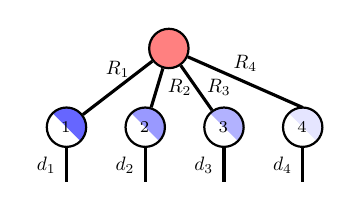
\begin{tikzpicture}[baseline=-0.5ex]
    \tikzset{tensor/.style = {minimum size = 0.5cm,shape = circle,thick,draw=black,inner sep = 0pt}, edge/.style = {thick,line width=.4mm},every loop/.style={}}
    \def\x{6}
    \def\y{0} 
    \node[tensor,fill=red!50!white] (G) at (\x+13.5,\y+1) {$\Gt$};
    \node[tensor, path picture={
    \fill[fill=blue!60!white](path picture bounding box.south east)
    -- 
    (path picture bounding box.north west) --
    (path picture bounding box.north east) -- cycle;
    }, shift={(\x+12.2,\y)}] (U_1)  {\scalebox{0.85}{$\Ub_1$}};  \node[tensor, path picture={
    \fill[fill=blue!40!white](path picture bounding box.south east)
    -- 
    (path picture bounding box.north west) --
    (path picture bounding box.north east) -- cycle;
    }, shift={(\x+13.2,\y)}] (U_2) {\scalebox{0.85}{$\Ub_2$}};
    \node[tensor, path picture={
    \fill[fill=blue!30!white](path picture bounding box.south east)
    -- 
    (path picture bounding box.north west) --
    (path picture bounding box.north east) -- cycle;
    }, shift={(\x+14.2,\y)}] (U_3) {\scalebox{0.85}{$\Ub_3$}};
        \node[tensor, path picture={
    \fill[fill=blue!10!white](path picture bounding box.south east)
    -- 
    (path picture bounding box.north west) --
    (path picture bounding box.north east) -- cycle;
    }, shift={(\x+15.2,\y)}] (U_4) {\scalebox{0.85}{$\Ub_4$}};
     \draw[edge] (U_1) -- (\x+12.2,\y-0.7) node [midway, left] {\scalebox{0.7}{\dimcolor{$d_1$}}};
    \draw[edge] (U_2) -- (\x+13.2,\y-0.7) node [midway, left] {\scalebox{0.7}{\dimcolor{$d_2$}}};
    \draw[edge] (U_3) -- (\x+14.2,\y-0.7) node [midway, left] {\scalebox{0.7}{\dimcolor{$d_3$}}};
    \draw[edge] (U_4) -- (\x+15.2,\y-0.7) node [midway, left] {\scalebox{0.7}{\dimcolor{$d_4$}}};
    \draw[edge](G) -- (U_1)node[midway,above]{\scalebox{0.7}{\dimcolor{$R_1$}}};
    \draw[edge](G) -- (U_2)node[midway,right]{\scalebox{0.7}{\dimcolor{$R_2$}}};
    \draw[edge](G) -- (U_3)node[midway,right]{\scalebox{0.7}{\dimcolor{$R_3$}}};
    \draw[edge](G) -- (\x+15.2,\y+0.25)node[midway,above]{\scalebox{0.7}{\dimcolor{$R_4$}}};
\end{tikzpicture}.
$$
其中张量 $\Gt = \Tt\ttm{1}\Ub_1^\ts\ttm{2}\dots\ttm{4}\Ub_4^\ts$。 

核心张量  $\Gt\in\RR^{R_1\times\dots\times R_4}$ 与因子矩阵 $\Ub_1,\dots,\Ub_4$ 一起构成张量 $\Tt$ 的一个 Tucker 分解。若 $\Tt$ 各矩阵化上的 SVD 全部精确，则所得的 Tucker 分解也是精确的。使用截断 SVD 时，Tucker 分解的整体逼近误差可表示为各截断 SVD 所引入误差的函数~(见~\citep{de2000multilinear})。

\paragraph{多重线性秩与矩阵化的秩}
上述算法表明：若对所有 $n$ 有 $\tilde R_n = \rank(\Tt_{(n)})$，则存在秩为 $(\tilde R_1,\dots, \tilde R_N)$ 的 Tucker 分解，这说明 $\Tt$ 的多重线性秩 $( R_1,\dots, R_N)$ 以矩阵化的秩为上界，即对所有 $n$ 有 $ R_n \leq \rank(\Tt_{(n)} )$。也容易证明，多重线性秩以矩阵化的秩为下界。事实上，设 $\T$ 的多重线性秩为 $(R_1,\dots, R_N)$，则存在秩 $(R_1,\dots, R_N)$ 的 Tucker 分解 $\Tt = \Gt\times_1\Ub_1\times_2 \dots \times_N \Ub_N$。由定理~\ref{thm: matricization-rank} 即可看出，这意味着对所有 $n$ 有 $\rank(\Tt_{(n)} )\leq  R_n$。
这就证明了如下定理。
\begin{theorem}
张量 $\Tt$ 的多重线性秩 $(R_1,R_2,\dots, R_N)$ 由其矩阵化的秩给出，即对 $n\in[N]$ 有 $R_n = \rank(\Tt_{(n)})$。
\end{theorem}


\begin{remark}\label{rem:tuckers}
这里列出 Tucker 分解以及用于计算它的高阶奇异值分解~(HOSVD) 算法的一些有趣性质。
\begin{enumerate}

\item  若 $\Tt = \Gt\ttm{1}\Ub_1\ttm{2}\dots\ttm{N-1}\Ub_{N-1}\ttm{N}\Ub_N$ 且所有 $\Ub_i$ 均正交，则 $\norm{\Tt}_F = \norm{\Gt}_F$，且 $\vectorize(\Gt) = (\Ub_1\kron\cdots\kron\Ub_N)\vectorize(\Tt)$。
事实上，当 $N=3$ 时有
\begin{align*}
(\Ub_1\kron\Ub_2\kron\Ub_3)\vectorize(\Tt) &= 
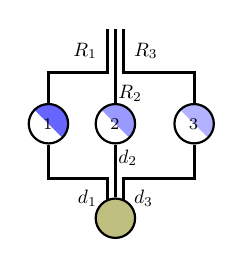
\begin{tikzpicture}[baseline=-0.5ex]
    \tikzset{tensor/.style = {minimum size = 0.5cm,shape = circle,thick,draw=black,inner sep = 0pt}, edge/.style = {thick,line width=.4mm},every loop/.style={}}
    \def\x{0}
    \def\y{0.5}   
    \node[tensor, path picture={
    \fill[fill=blue!60!white](path picture bounding box.south east)
        -- 
    (path picture bounding box.north west) --
    (path picture bounding box.north east) -- cycle;
    }, shift={(\x-0.85,\y-0.65)}] (U_1) {\scalebox{0.85}{$\Ub_1$}};
    \node[tensor, path picture={
    \fill[fill=blue!40!white](path picture bounding box.south east)
        -- 
    (path picture bounding box.north west) --
    (path picture bounding box.north east) -- cycle;
    }, shift={(\x,\y-0.65)}] (U_2) {\scalebox{0.85}{$\Ub_2$}};
    \node[tensor, path picture={
    \fill[fill=blue!30!white](path picture bounding box.south east)
        -- 
    (path picture bounding box.north west) --
    (path picture bounding box.north east) -- cycle;
    }, shift={(\x+1,\y-0.65)}] (U_3) {\scalebox{0.85}{$\Ub_3$}};
    \draw[edge] (U_1) -- (\x-0.85,\y-1.35) -- (\x-0.1,\y-1.35) -- (\x-0.1,\y-1.85) node [midway, left] {\scalebox{0.7}{\dimcolor{$d_1$}}};
    \draw[edge] (U_2) -- (\x,\y+0.55) node [very near start, right=-0.1cm] {\scalebox{0.7}{\dimcolor{$R_2$}}};
    \draw[edge] (U_3) -- (\x+1,\y-1.35) -- (\x+0.1,\y-1.35) -- (\x+0.1, \y-1.85) node [midway, right] {\scalebox{0.7}{\dimcolor{$d_3$}}};
    \draw[edge](U_1) -- (\x-0.85,\y) -- (\x-0.1,\y) -- (\x-0.1,\y+0.55)node [midway, left] {\scalebox{0.7}{\dimcolor{$R_1$}}};
    \draw[edge](U_3) -- (\x+1,\y) -- (\x+0.1,\y) -- (\x+0.1,\y+0.55)node [midway, right] {\scalebox{0.7}{\dimcolor{$R_3$}}};
    \node[tensor,fill=green!50!red!50!white](T) at (\x,\y-1.85) {$\Tt$};
    \draw[edge](U_2)--(T)node [near start, right=-0.1cm] {\scalebox{0.7}{\dimcolor{$d_2$}}};
\end{tikzpicture}
=
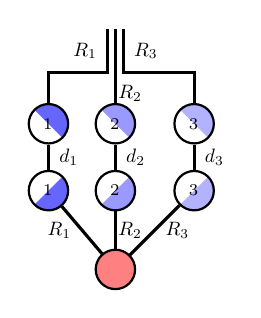
\begin{tikzpicture}[baseline=-0.5ex]
    \tikzset{tensor/.style = {minimum size = 0.5cm,shape = circle,thick,draw=black,inner sep = 0pt}, edge/.style = {thick,line width=.4mm},every loop/.style={}}
    \def\x{0}
    \def\y{1.25}   
    \node[tensor, path picture={
    \fill[fill=blue!60!white](path picture bounding box.south east)
        -- 
    (path picture bounding box.north west) --
    (path picture bounding box.north east) -- cycle;
    }, shift={(\x-0.85,\y-0.65)}] (U_1) {\scalebox{0.85}{$\Ub_1$}};
    \node[tensor, path picture={
    \fill[fill=blue!60!white](path picture bounding box.north east)
        -- 
    (path picture bounding box.south west) --
    (path picture bounding box.south east) -- cycle;
    }, shift={(\x-0.85,\y-1.5)}] (Ut_1) {\scalebox{0.85}{$\Ub_1$}};
    \node[tensor, path picture={
    \fill[fill=blue!40!white](path picture bounding box.south east)
        -- 
    (path picture bounding box.north west) --
    (path picture bounding box.north east) -- cycle;
    }, shift={(\x,\y-0.65)}] (U_2) {\scalebox{0.85}{$\Ub_2$}};
     \node[tensor, path picture={
    \fill[fill=blue!40!white](path picture bounding box.north east)
        -- 
    (path picture bounding box.south west) --
    (path picture bounding box.south east) -- cycle;
    }, shift={(\x,\y-1.5)}] (Ut_2) {\scalebox{0.85}{$\Ub_2$}};
    \node[tensor, path picture={
    \fill[fill=blue!30!white](path picture bounding box.south east)
        -- 
    (path picture bounding box.north west) --
    (path picture bounding box.north east) -- cycle;
    }, shift={(\x+1,\y-0.65)}] (U_3) {\scalebox{0.85}{$\Ub_3$}};
    \node[tensor, path picture={
    \fill[fill=blue!30!white](path picture bounding box.north east)
        -- 
    (path picture bounding box.south west) --
    (path picture bounding box.south east) -- cycle;
    }, shift={(\x+1,\y-1.5)}] (Ut_3) {\scalebox{0.85}{$\Ub_3$}};
    \draw[edge] (U_2) -- (\x,\y+0.55) node [very near start, right=-0.1cm] {\scalebox{0.7}{\dimcolor{$R_2$}}};
    \draw[edge](U_1) -- (\x-0.85,\y) -- (\x-0.1,\y) -- (\x-0.1,\y+0.55)node [midway, left] {\scalebox{0.7}{\dimcolor{$R_1$}}};
    \draw[edge](U_3) -- (\x+1,\y) -- (\x+0.1,\y) -- (\x+0.1,\y+0.55)node [midway, right] {\scalebox{0.7}{\dimcolor{$R_3$}}};
    \draw[edge](U_1)--(Ut_1)node [midway, right] {\scalebox{0.7}{\dimcolor{$d_1$}}};
    \draw[edge](U_2)--(Ut_2)node [midway, right] {\scalebox{0.7}{\dimcolor{$d_2$}}};
    \draw[edge](U_3)--(Ut_3)node [midway, right] {\scalebox{0.7}{\dimcolor{$d_3$}}};
    \node[tensor,fill=red!50!white] (G) at (\x,\y-2.5) {$\Gt$};
    \draw[edge](G)--(Ut_1)node [midway, left] {\scalebox{0.7}{\dimcolor{$R_1$}}};
    \draw[edge](G)--(Ut_2)node [midway, right=-0.1cm] {\scalebox{0.7}{\dimcolor{$R_2$}}};
    \draw[edge](G)--(Ut_3)node [midway, right] {\scalebox{0.7}{\dimcolor{$R_3$}}};
\end{tikzpicture}
=
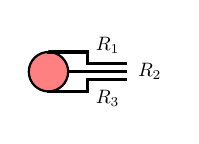
\begin{tikzpicture}[baseline=-0.5ex]
    \tikzset{tensor/.style = {minimum size = 0.5cm,shape = circle,thick,draw=black,inner sep = 0pt}, edge/.style = {thick,line width=.4mm},every loop/.style={}}
    \def\x{6}
    \def\y{0}
    \node[tensor,fill=red!50!white] (G) at (\x+4.5,\y) {$\Gt$};
    \draw[edge](G) -- (\x+5.5,\y) node [right] {\scalebox{0.7}{\dimcolor{$R_2$}}};
    \draw[edge](G) -- (\x+4.5,\y+0.25) -- (\x+5,\y+0.25) -- (\x+5,\y+0.1) -- (\x+5.5, \y+0.1) node [midway,above] {\scalebox{0.7}{\dimcolor{$R_1$}}};
    \draw[edge](G) -- (\x+4.5,\y-0.25) -- (\x+5,\y-0.25) -- (\x+5,\y-0.1) -- (\x+5.5, \y-0.1) node [midway,below] {\scalebox{0.7}{\dimcolor{$R_3$}}};
    \end{tikzpicture}
    =\vectorize(\Gt).
\end{align*}

